\documentclass[12pt]{article}
\usepackage[dvips]{epsfig}
\usepackage{color}
%e.g.  \textcolor{red,green,blue}{text}
\usepackage{url}
\usepackage[colorlinks=true]{hyperref}

\begin{document}

\section*{GENESIS: Documentation}

\section*{Unix and the Linux Graphical Desktop}

After you have logged in, you will be presented with a desktop showing several icons and a panel that is similar to the Windows taskbar. It is usually located at the bottom of the screen, but could also be located at the top, or even one of the sides. Linux and its graphical interface, the X window system, give a lot of choices and configuration options for the desktop environment. The most commonly used desktops are the KDE desktop and the GNOME desktop.

For KDE, the panel may look something like this

\begin{figure}[h]
  \centering
 
\includegraphics[scale=0.35]{figures/kde-gnxbar.eps}
  %\caption{enumerate}
  \label{fig:kde-gnxbar}
\end{figure}

or with GNOME, it might look like this

\begin{figure}[h]
  \centering
 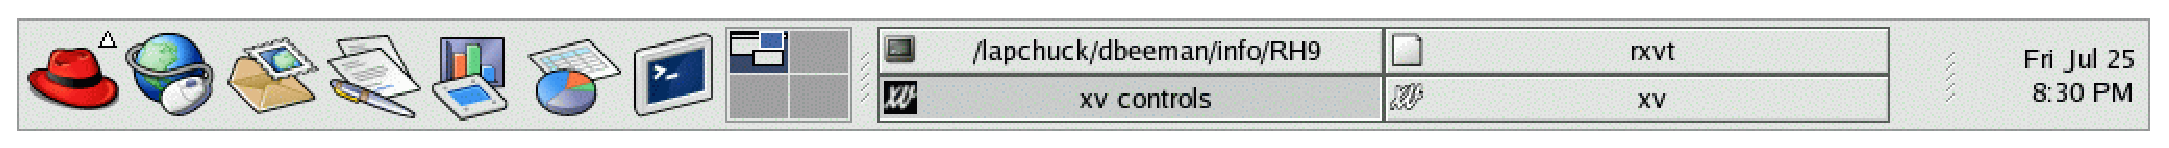
\includegraphics[scale=0.35]{figures/gnomebar-term.eps}
  %\caption{enumerate}
  \label{fig:gnomegnxbar}
\end{figure}

Some of the more important icons that you can click on are the

%\begin{wrapfigure}[lineheight]{alignment}{width}
\begin{quote}
	
\includegraphics[width=0.05\textwidth]{figures/redhat-main-menu32.eps} {\bf Red Hat main menu}\\
	 
\includegraphics[width=0.05\textwidth]{figures/kmenu.eps} {\bf KDE main menu}\\
	 
\includegraphics[width=0.05\textwidth]{figures/gnome-logo-icon32.eps} {\bf GNOME main menu}\\
	 Like the MS Windows start menu, these may be used to logout or to select programs to run (some of which are in sub-menus). They are usually located at the left end of the control panel (see the GNOME and KDE panel figures above).

\end{quote}

\begin{quote}
	
\includegraphics[width=0.05\textwidth]{figures/konsole.eps} {\bf KDE Terminal window} \\
	
\includegraphics[width=0.05\textwidth]{figures/gnome-term.eps}{\bf UNIX Terminal window}

This is a console window that allows you to type commands to the UNIX shell. It is one of the most important applications in UNIX and Linux. Once you get used to it, you will find that after learning a few cryptic two-letter UNIX/Linux commands, you will get things done much faster than going through many levels of sub-menus with a GUI. You will create and run GENESIS simulations by giving commands in a terminal window.

Note that if your taskbar doesn't have an icon for a terminal window, look for it in the System Tools sub-menu of the Main Menu.
\end{quote}

\begin{quote}
	
\includegraphics[width=0.05\textwidth]{figures/konsole.eps} {\bf Web browser} (often Mozilla).\\
	The bookmark feature of the browser can be used to set bookmarks for GENESIS and other documentation.

	
\includegraphics[width=0.05\textwidth]{figures/konqueror.eps} {\bf Konqueror}.\\
	A fast and light-weight web browser provided wth KDE that is good for reading documentation.

	
\includegraphics[width=0.05\textwidth]{figures/khelpcenter.eps} {\bf KDE help center }\\
	Provides links to information about the KDE desktop environment, KDE applications on the KDE start menu, the UNIX manual (``man") pages, and GNU ``info" documentation.

	
\includegraphics[width=0.05\textwidth]{figures/kcontrol.eps} {\bf KDE control center}\\
	Used for changing the configuration of the KDE desktop environment.
	
	
\includegraphics[width=0.05\textwidth]{figures/desktops.eps} {\bf Desktops display}\\
	Most Linux desktop environments allow you to switch between multiple desktops, so that your screen doesn't become too cluttered with applications and terminal windows. For example, you could be running a GENESIS simulation on one desktop, have a couple of browser windows open on another, and be editing two or three files on a third. Here, the taskbar has been configured to let you switch between four desktops by clicking on one with the mouse. 
\end{quote}

\subsection*{Getting around in UNIX and Linux}

The commands that you type within a terminal window are interpreted by a {\it UNIX shell}. Your account will have been set up to use a particular default shell. The most common shell used with Linux is {\it bash}, a variation of the Bourne shell {\it sh}. Some prefer to use {\it tcsh}, a variation of the Berkeley C shell {\it csh}. All of these shells recognize the same common commands described below for creating, navigating, or copying files between directories (in Mac/Windows-speak, ``folders").

When you first bring up a terminal window, you are placed in your home directory. A few default configuration files with names starting with ``{\it .}'' have been set up for you, but otherwise your directory is empty (as file names starting with ``{\it .}'' are not visible in a file manager GUI--but see below). You can get a listing of the current directory by using the {\it ls} command (short for ``list''). This is like the DOS {\it dir} command, but you need to specify some options (followed by a dash) to get details. To get a more detailed listing (including the otherwise invisible ``dot files"), type ``{\tt ls -lags}".

To traverse to another directory you use the {\it cd} (change directory) command. This command takes an argument of the directory you wish to change to. Either an absolute or relative path argument can be specified. Absolute paths begin at the ``root" of the UNIX file system (``/''). Relative paths begin from the currect working directory. For example, if you are in your home directory, you can get to a next lower directory, e.g. {\it genesis}, by typing ``{\tt cd genesis}". Typing ``{\tt cd}" by itself changes you directly to your home directory. The following shorthand symbols can be used to refer to commonly used directories:

\begin{quote}
	$\sim$ Your home directory.
	
	{\tt\bf .} The directory that you are currently in (``current working directory").
	
	 {\tt\bf ..} The directory immmediately above the current working directory. 
\end{quote}

To create a directory, use the {\it mkdir} command, e.g. ``{\tt mkdir myScripts}". Note that file and directory names in UNIX are case-sensitive so ``{\tt mkdir myScripts}" is not the same as ```{\tt mkdir myscripts}".

To print the name of the current working directory you can use the {\it pwd} (print working directory) command.

You can examine text files (such as all of our README files) using the {\it more} command. This command will display a screenful of lines at a time. Pressing the space bar on your keyboard displays the next screen full of lines, and pressing ``b" takes you back one screenful. Pressing ``Enter" displays one additional line. Pressing ``\ '\ '' (apostrophe) returns you to the top of the file and ``q" will exit the {\it more} command. For example, ``{\tt more tutorial1.g}'' will display the contents of the file ``tutorial1.g'' if it exists in the current working directory. The ``pipe'' symbol ``\,$|$\,'' can be used to send the output of one command into another. For example, try the command ``{\tt ls -lags $\sim$ | more}''.

Other useful commands are {\it rm}, meaning remove or delete, as in ``{\tt rm junk.mail}'', and {\it cp} to copy one file into another, as in ``{\tt cp tutorial3.g $\sim$/myScripts/tutorials}''. The ``{\tt -r}'' option lets you recursively copy a directory with its contents, including any subdirectories. For example, if GENESIS is installed in ``/usr/local/genesis'', to make your copy of the {\it genesis/Scripts/tutorials} directory, you would type
\begin{verbatim}
  cd /usr/local/genesis/Scripts
  cp -r tutorials ~/myScripts
 \end{verbatim}
The {\it mv} command is used to rename a file or move it to a different directory, instead of copying it.

The two most common text editors for UNIX are {\it vi} and {\it emacs}. If you are not familiar with either editor, you may find it easier to learn \href{http://www.gnu.org/software/emacs/tour/}{\it emacs}. For an even simpler text editor with built-in help, try \href{http://www.nano-editor.org/}{\it nano} if it is installed. If you are using Linux with the KDE or GNOME desktop, try \href{http://webcvs.kde.org/kdeutils/kedit/}{\it kedit} or \href{http://projects.gnome.org/gedit/}{\it gedit}.

Documentation for most UNIX commands can be obtained with the {\it man} command. For example ``{\tt man ls}" will tell you about all the options for the {\it ls} command.

The main source for Linux information is \href{http://www.tldp.org/ }{The Linux Documentation Project}.

If most of this is new to you, now would be a good time to open a terminal window and try out some of the commands described above.

\end{document}
\end{document}
